
\chapter{Medizinische Grundlagen}\label{chap:Medizinische_Grundlagen}
\section{Symptom}
Periodische Gliedmaßenbewegungen (\acrshort{PLM}) sind wiederholte Bein- oder seltener Armbewegungen, die ein- oder beidseitig auftreten und symmetrisch oder alternierend sein können. Sie treten meist nach einer typischen Beugung der großen Gelenke (Hüfte, Knie, Sprunggelenk) und Streckung der großen Zehe auf. Zu beobachten ist dieses Symptom episodisch meist beim Übergang zwischen dem Wachzustand und dem oberflächlichen Schlaf (Schlafphase N1) und im stabilen Leichtschlaf (Schlafphase N2), aber auch in Ruhephasen im Wachzustand. Die Auftretenswahrscheinlichkeit nimmt mit dem Alter zu und versechsfacht sich ab dem 50. Lebensjahr auf circa 30 Prozent. \cite{PDS}

Die relevantesten Definitionen über periodische Beinbewegungen (PLM) im Schlaf kommen von der \gls{AASM} und der World Association of Sleep Medicine, welche Beinbewegungen und deren periodisches Auftreten quantitativ beschreiben. Die Kriterien und Zahlenwerte sind sich weitestgehend ähnlich \cite{worldsleepcongress}. Diese Arbeit stützt sich auf die Kriterien der AASM (2016) \cite{AASM}:
\begin{enumerate}
	\item Das Signal der Elektromyographie (EMG) sollte bei entspanntem Tibialis anterior-Muskel bestimmt werden 
    \item Der Beginn des LM wird festgelegt, wenn die Zunahme des EMGs acht Mikrovolt über dem Ruhesignal liegt. Das Ende des LM wird bei einer Reduktion des EMG-Signals auf weniger als zwei Mikrovolt über dem Ruhesignal für mindestens 0.5 Sekunden festgelegt.
    \item Die zeitliche Dauer eines LM liegt zwischen minimal 0.5 Sekunden und maximal zehn Sekunden.
    \item Beinbewegungen an zwei unterschiedlichen Beinen werden dann als eine zusammenhängende LM klassifiziert, wenn weniger als fünf Sekunden zwischen den Anfängen beider Bewegungen liegen. 
    \item Als periodisch gelten mindestens vier LM, die jeweils innerhalb eines Zeitraumes zwischen fünf und 90 Sekunden aufeinander folgen.
    \item Sie werden in allen Schlafstadien und im Wachzustand bestimmt.
    \item Leg Movements am Ende einer Apnoe oder Hypopnoe, die gemeinsam mit dem Hyperventilationsbeginn auftraten, werden nicht bewertet, wenn sie in einem Zeitfenster auftreten, das 0.5 Sekunden vor dem Anfang einer Apnoe oder Hypopnoe beginnt und 0.5 Sekunden nach dem Ende einer Apnoe oder Hypopnoe endet
\end{enumerate}
Die Kriterien wurden evidenzbasiert getroffen, basierten auf Literatur-Reviews oder auf Konsensverfahren \cite{PDS}. Zur Übersicht wurden die Abbildung \ref{fig:AASMKrit} erstellt.
\begin{figure}[!ht]%
	\begin{center}
	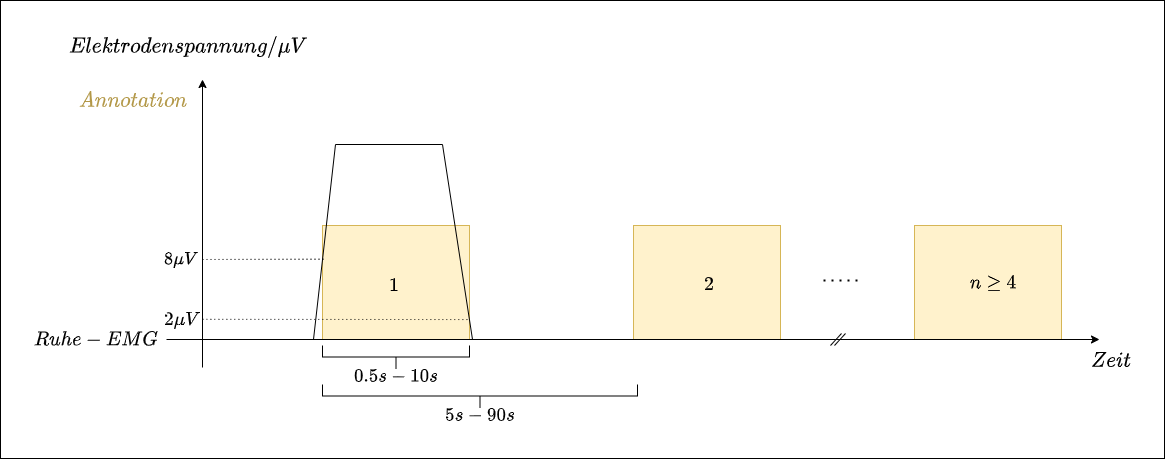
\includegraphics[width=0.80\textwidth]{./Bilder/AASMLM.drawio (2).png}
	\end{center}
	\caption{Graphische Veranschaulichung der AASM-Kriterien.}%
	\label{fig:AASMKrit}%
\end{figure}
Die Muskelaktivität spielt auch bei folgenden Symptomen eine Rolle, muss aber von diesen abgegrenzt werden: hypnagogem Fußzittern (Hypnagogic Foot Tremor), alternierender Beinmuskelaktivität (Alternating Leg Muscle Activation, ALMA), exzessivem fraktionierten Myoklonus im NonREM-Schlaf, phasischen REM-twitches und Wadenkrämpfen \cite{PDS}. Die Kriterien zur Unterscheidung von anderen Bewegungsstörungen sind in \cite{AASM} beschrieben.

Die Beinbewegungen können mit Arousals einher gehen, welche zu einer partiellen, temporären oder vollständigen Weckreaktion führen. Diese äußern sich durch eine abrupte Frequenzänderung im Elektroenzephalogramm und sollen, laut der AASM, den Beinbewegungen zugeordnet werden. Da die Beinbewegungen überwiegend in den Schlafstadien N1 und N2 auftreten und oft mit Weckreaktionen einhergehen, sind REM- und Tiefschlaf häufig vermindert. Darunter leidet die Schlafeffizienz und die gesunde Periodizität der Schlafphasen wird gestört. Bei länger anhaltenden Beschwerden entwickeln viele Patienten zusätzlich psychische Fehlhaltungen und Verhaltensweisen, die die Schlafqualität weiter verschlechtern. Der Schlaf ist dadurch weniger erholsam. Es kommt zu Symptomen einer Hypersomnie, wie zum Beispiel eine ausgeprägte Tagesschläfrigkeit und Monotonieintoleranz sowie sekundäre depressive Symptome, imperative Einschlafattacken, Gedächtnis- und Aufmerksamkeitsstörungen. Diese können den Alltag stark beeinträchtigen und beispielsweise beim Autofahren sogar tödlich sein. Darüber hinaus werden die PLM mit Herzkrankheiten, hohem Blutdruck und Herzversagen assoziiert \cite{Huang}. \cite{PDS}

In der Praxis wird der PLMS-Index, also die Anzahl der pro Stunde auftretenden periodischen Beinbewegungen im Schlaf, genutzt, um das Ausmaß einer möglichen Erkrankung festzustellen. Dabei gelten bis zu fünf pro Stunde als unauffällig, zwischen fünf pro Stunde und ≤20 pro Stunde als leichte Störung, zwischen 20 pro Stunde und 60 pro Stunde als moderate Störung und bei einem PLMS-Index über 60 pro Stunde als schwere Erkrankung. \cite{PDS}


\section{Ursachen}
Periodische Beinbewegungen sind Symptome vieler unterschiedlicher Krankheiten. Diese treten beim \gls{RLS} in 80 Prozent der Fälle, bei der REM-Verhaltensstörung in 70 Prozent und bei Narkolepsie in 45 Prozent bis 60 Prozent der Fälle auf. Bei der Krankheit Insomnie sind in 1 Prozent bis 15 Prozent der Fälle periodische Beinbewegungen symptomatisch und bei einer obstruktiven Schlafapnoe sind auch oft PLM vorhanden. Außerdem werden diese häufig in Assoziation mit psychiatrischen Störungen und bei neurologischen Erkrankungen wie Multisystematrophie oder Rückenmarksverletzungen gefunden. Auch Nebenwirkungen durch eingenommene Medikamente sind möglich. Dies ist allerdings nur eine Auswahl aller möglichen Ursachen. Falls das Symptom nicht durch eine der obigen Krankheiten erklärt werden kann, wird die Diagnose "Periodic-Limb-Movement-Disorder" gestellt, auch wenn die Krankheiten simultan auftreten können \cite{1x1}. \cite{PDS}

Da die Krankheitsbilder sehr unterschiedlich sind, sind auch die Ursachen für periodische Beinbewegungen vielfältig. Bei dem RLS und PLMD ist die Erkrankung ähnlich, aber noch weitgehend unverstanden. Diese entsteht wahrscheinlich im Zentralnervensystem durch eine Störung des dopaminergen oder opioidergen Systems \cite{1x1}, welche durch eine Störung des Eisenstoffwechsels auftreten könnte. Diese These wird gestützt durch das vermehrte Auftreten von PLM im höheren Alter bei einem gleichzeitigen Verlust an Dopamin und Dopaminrezeptoren. Die mit RLS korrelierenden Gene könnten auf eine frühe Entwicklungsstörung des zentralen Nervensystems hindeuten. \cite{PDS}

\section{Therapie}

Periodische Beinbewegungen sollen nur dann behandelt werden, wenn sie eine Insomnie oder Hypersomnie auslösen, welche nicht durch andere Erkrankungen erklärt werden kann. Grundsätzlich gilt, dass nach Möglichkeit zuerst die Grunderkrankung behandelt werden sollte, falls diese in Verbindung mit PLM auftritt. \cite{PDS}

Das RLS und PLMD werden pharmakologisch behandelt, indem die oben beschriebenen Mängel ausgeglichen werden. Hier soll zuerst dopaminerg, danach antiepileptisch und als letzte Maßnahme opioiderg behandelt werden. Hier eignen sich die Wirkstoffe L-Dopa, Rotigotin und Oxycodon je nach Schweregrad. Zusätzlich ist eine Eisensubstitution empfehlenswert. Insomnien sollten generell mit nichtmedikamentösen Verfahren kombiniert werden, indem über Grundlagenwissen der Schlafhygiene (z.B. Zubettgeh-Ritual, Matratze, Raumtemperatur, Geräuschisolierung und Abdunkelungsmöglichkeiten) aufgeklärt wird. Die Verwendung von schlaffördernden Mitteln wirkt lediglich symptomatisch und sollte nur über einen begrenzten Zeitraum erfolgen. \cite{1x1,PDS}

Die meisten Krankheitsbilder werden in erster Linie durch Fragebögen festgestellt. Die periodischen Beinbewegungen werden jedoch in der Regel nicht durch den Patienten in der Nacht wahrgenommen. Eine mögliche schlafstörende Wirkung kann durch ein Elektroenzephalogramm bestätigt werden. Dies ist nötig, da sonst keine Therapie verschrieben werden darf. Bei diagnostisch unklaren Fällen, sowie bei Kindern und Jugendlichen kann es auch gerechtfertigt sein, den Schlaf im Schlaflabor zu überwachen. \cite{1x1}


\section{Biophysikalischer Signalursprung}

In der folgenden Arbeit werden Daten aus Elektromyogrammen ausgewertet. Deswegen ist es an dieser Stelle wichtig, zu verstehen, welchen biophysikalischen Ursprung die ausgewerteten Signale haben. 
Da Beinbewegungen im PSG nicht direkt gemessen werden können, werden im Schlaflabor ersatzweise die Muskelkontraktionen des Beines gemessen, welche die Bewegungen verursachen. Um in diesem Kontext eine Muskelkontraktion zu verursachen, muss zunächst ein Signal in Form eines Aktionspotentials einer Nervenzelle zu dem Muskel weitergeleitet werden. Diese Nervenzelle bewirkt eine Depolarisation in der anliegenden Muskelzelle, in der Calciumionen freigesetzt werden \cite{biomechanist}. Die Calciumionen ermöglichen dann die Kontraktion des Muskels \cite{motorischeEndplatte}. Dieser Vorgang verändert das Potentialfeld, welches an der Hautoberfläche mit einer Elektrode gemessen werden kann. Die Änderung ergibt sich aus der Überlagerung der Depolarisation von Nerven- und Muskelzellen, welche anschließend durch aktives Zurückpumpen von Calciumionen repolarisiert werden \cite{motorischeEndplatte}. Da Muskeln aus vielen Fasern bestehen, welche jeweils nur kurz und mehrfach an einer Kontraktion des gesamten Muskels beteiligt sind, ist die Potentialänderung ein stochastisches Signal in einem Frequenzbereich von zwischen zehn Hertz und 500 Hertz \cite{Mehrkanal-BioimpedanzInstrumentierung}. Die ein bis drei Quadratmillimeter große Depolarisationszone wird mit einer Geschwindigkeit von zwei bis sechs Meter pro Sekunde entlang der Muskelfaser weitergeleitet \cite{biomechanist}.
Laut AASM sollen die Kontraktion beider Beine anhand jeweils zweier Elektroden gemessen werden, welche entlang des Tibialis Anterior Muskels (Tibialis anterior muscle) platziert sind \cite{AASM}. 

\section{Störgrößen}
Der Vorteil in der Nutzung zweier Elektroden ergibt sich aus der verbesserten Unterdrückung von Störgrößen. Das Signal ist dadurch im Idealfall unabhängig von Einflussgrößen, welche auf beide Elektroden wirken und daher nicht von dem gewünschten Signal verursacht wurden. Diese Störgrößen beinhalten das statische Potentialfeld, Haut-Elektrode Übergänge, kapazitive und induktive Einkopplung von anderen elektrischen Geräten und der Netzspannung. 
Im Idealfall heben sich die Halbzellspannungen auf, welche durch den Elektrode-Haut-Übergang entstehen. Die oben genannten Gleichtaktstörgrößen beeinflussen das Signal jedoch wenig, falls die Bioimpedanzen klein sind im Vergleich zu der Innenimpedanz des Messinstruments. Die AASM empfiehlt Impedanzen von 5000 Ohm \cite{AASM}. \cite{Mehrkanal-BioimpedanzInstrumentierung}

Problematisch sind auch zeitliche Änderung der Haut-Elektrode Übergänge, welche durch die Bewegung oder Schweiß entstehen können \cite{Mehrkanal-BioimpedanzInstrumentierung,PRT}.
Zwischen dem Muskel und der Elektrode befindet sich weiteres Gewebe, welches das Signal nichtlinear verzerren kann und wie ein Tiefpass Filter wirkt, dessen Grenzfrequenz mit der Gewebedicke abnimmt. Eine weitere Störgröße ist die Überlagerung von Potentialfeldern, welche durch das Herz oder die Atmung verursacht wurden \cite{Moore,1x1}. \cite{physiology}

Das Schlafverhalten des Patienten ist möglicherweise aufgrund der Verkabelung und Überwachung im Schlaflabor gestört \cite{1x1}. Zudem kann es selbst bei einer schweren Erkrankung Nächte geben, in denen wenig periodische Beinbewegungen auftreten \cite{PDS}.
